\renewcommand{\abstractname}{Executive Summary}
\begin{abstract}
    The field of quadruped robotics, or the study of 4-legged robots, has been inspired by the limitation of wheeled and tracked robotic systems. Walking robots generally excel in rocky uneven terrain for search and rescue and disaster relief operations. Therefore, as technology increases, quadrupeds have a huge potential to be used where other robots and/or humans can’t go. However, research in walking robotics is hard to do, partially because there is not a ubiquitous platform for research and development. The few research quadrupeds include Boston Dynamics’ Spot Mini and Tekken, and cost hundreds of thousands of dollars to build. SmallKat MQP’s robot is designed to be a quadrupedal robotic platform to help research and design new gaits, test sensors, and teach engineering students.
    
    In order for it to be a successful research platform, SmallKat needed to be balanced and powerful, while maintaining configurability. It also needed to be easily manufacturable and adaptable to change to allow users to modify any parts and add additional components and sensors. Therefore, we chose to design this robot to be built using additive manufacturing techniques on consumer 3D printers. For maximum adaptability, the 4-DoF legs are powered by standard sized servos (JX HV-5932MG) with custom motor controllers built into the servo casing. We chose 4 degrees of freedom since our particular configuration allowed us to customize the angle to the ground for optimal grip when walking. The molded polyurethane feet add an increased coefficient of friction with the ground and have integrated pressure sensors to measure the force vector produced when contacting the ground. Finally, we added an advanced continuum tail powered by 4 Maxon motors and a 2-DoF head for better control over balance when dynamically walking.
    \begin{figure}[H]
        \centering
        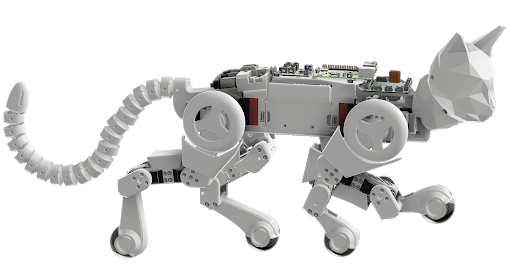
\includegraphics[width=0.9\textwidth]{figures/FinalDesign.png}
        \caption{The SmallKat Quadrupedal Robotics Research Platform}
        \label{fig:ExecutiveSummaryRobot}
    \end{figure}
    
    We also developed custom electronics and a communication stack that was optimized for high-speed data transfer between our motors and sensors. The motor controllers developed were integrated inside the servo casing and ran a PID controller for the position, velocity, and torque at over 10kHz. We also developed custom foot sensors that measured the force vector from impact with the feet in order to provide feedback for advanced waking gaits in rough terrain. In order to effectively communicate on the same communication stack, a custom charger was developed for the battery, as well as a driver and controller for the continuum tail and a 9-DoF inertial measurement board for feedback into higher level controllers. This was all tied together via a custom motherboard running a 400 MHz micro controller that connected all the boards together.
    \begin{figure}[H]
        \centering
        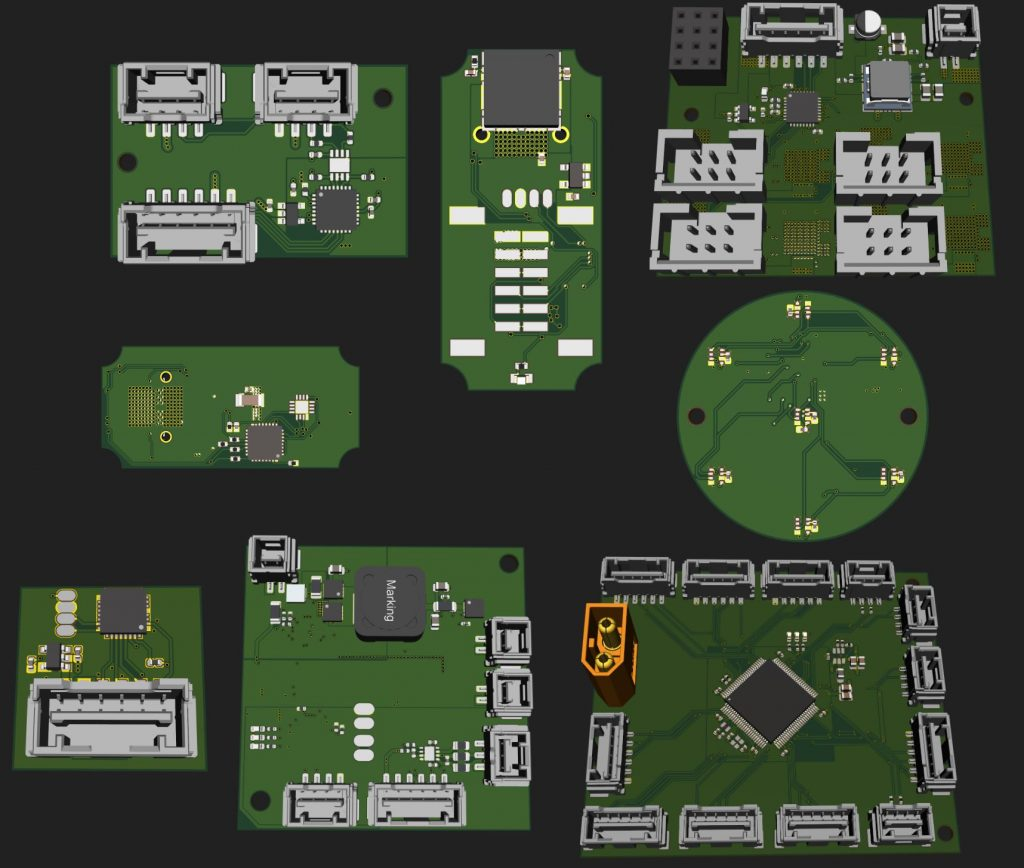
\includegraphics[width=0.9\textwidth]{figures/Electronics.jpg}
        \caption{Electronics Integrated in SmallKat}
        \label{fig:ExecutiveSummaryElectronics}
    \end{figure}
    These controllers were all tied together using a custom communication stack. SPI was used for communication between the motherboard and the IMU, the charger, the foot sensors, and the tail. To prevent having too many wires, RS485 was used to communicate with the motors in the legs and the head. Then, the motherboard relayed all this information back over USB HID to the Raspberry Pi 3 B+, which ran kinematics and dynamics calculations as well as the walking gaits. The software running on the Raspberry Pi 3 also had the capability to be controlled over WIFI to allow for wireless testing.
    The Raspberry Pi 3 performed kinematics and dynamics calculations using Bowler Kernel as a software platform. This allowed us to use previously developed basic walking gaits when testing. We also used Bowler Studio as a development environment, which included a simulator to test any kinematics and gaits before running on the robot. The kinematics and some dynamics were developed through this project, and a basic walking gait was tuned and tested. We also started the development of a more complex dynamic walking gait which used a central pattern generator for trajectory generation and calculated stability using the Wide Stability Margin.
    
    In the end, a 4-DoF quadrupedal platform was designed using custom sensors, motor controllers, and accessory boards. SmallKat also walked its first steps using the walking gait developed. In the future, we would like to see the dynamic walking gait be developed, as well as revisions for the robot as a whole, including the electronics and mechanical design. Future research can also look more carefully at the advantages of using a 4-DoF leg over a 3-DoF leg in quadrupeds.
\end{abstract}
